% Options for packages loaded elsewhere
\PassOptionsToPackage{unicode}{hyperref}
\PassOptionsToPackage{hyphens}{url}
%
\documentclass[
  ignorenonframetext,
]{beamer}
\usepackage{pgfpages}
\setbeamertemplate{caption}[numbered]
\setbeamertemplate{caption label separator}{: }
\setbeamercolor{caption name}{fg=normal text.fg}
\beamertemplatenavigationsymbolsempty
% Prevent slide breaks in the middle of a paragraph
\widowpenalties 1 10000
\raggedbottom
\setbeamertemplate{part page}{
  \centering
  \begin{beamercolorbox}[sep=16pt,center]{part title}
    \usebeamerfont{part title}\insertpart\par
  \end{beamercolorbox}
}
\setbeamertemplate{section page}{
  \centering
  \begin{beamercolorbox}[sep=12pt,center]{part title}
    \usebeamerfont{section title}\insertsection\par
  \end{beamercolorbox}
}
\setbeamertemplate{subsection page}{
  \centering
  \begin{beamercolorbox}[sep=8pt,center]{part title}
    \usebeamerfont{subsection title}\insertsubsection\par
  \end{beamercolorbox}
}
\AtBeginPart{
  \frame{\partpage}
}
\AtBeginSection{
  \ifbibliography
  \else
    \frame{\sectionpage}
  \fi
}
\AtBeginSubsection{
  \frame{\subsectionpage}
}
\usepackage{lmodern}
\usepackage{amssymb,amsmath}
\usepackage{ifxetex,ifluatex}
\ifnum 0\ifxetex 1\fi\ifluatex 1\fi=0 % if pdftex
  \usepackage[T1]{fontenc}
  \usepackage[utf8]{inputenc}
  \usepackage{textcomp} % provide euro and other symbols
\else % if luatex or xetex
  \usepackage{unicode-math}
  \defaultfontfeatures{Scale=MatchLowercase}
  \defaultfontfeatures[\rmfamily]{Ligatures=TeX,Scale=1}
\fi
% Use upquote if available, for straight quotes in verbatim environments
\IfFileExists{upquote.sty}{\usepackage{upquote}}{}
\IfFileExists{microtype.sty}{% use microtype if available
  \usepackage[]{microtype}
  \UseMicrotypeSet[protrusion]{basicmath} % disable protrusion for tt fonts
}{}
\makeatletter
\@ifundefined{KOMAClassName}{% if non-KOMA class
  \IfFileExists{parskip.sty}{%
    \usepackage{parskip}
  }{% else
    \setlength{\parindent}{0pt}
    \setlength{\parskip}{6pt plus 2pt minus 1pt}}
}{% if KOMA class
  \KOMAoptions{parskip=half}}
\makeatother
\usepackage{xcolor}
\IfFileExists{xurl.sty}{\usepackage{xurl}}{} % add URL line breaks if available
\IfFileExists{bookmark.sty}{\usepackage{bookmark}}{\usepackage{hyperref}}
\hypersetup{
  pdftitle={METARET},
  pdfauthor={Paolo Crosetto},
  hidelinks,
  pdfcreator={LaTeX via pandoc}}
\urlstyle{same} % disable monospaced font for URLs
\newif\ifbibliography
\usepackage{graphicx,grffile}
\makeatletter
\def\maxwidth{\ifdim\Gin@nat@width>\linewidth\linewidth\else\Gin@nat@width\fi}
\def\maxheight{\ifdim\Gin@nat@height>\textheight\textheight\else\Gin@nat@height\fi}
\makeatother
% Scale images if necessary, so that they will not overflow the page
% margins by default, and it is still possible to overwrite the defaults
% using explicit options in \includegraphics[width, height, ...]{}
\setkeys{Gin}{width=\maxwidth,height=\maxheight,keepaspectratio}
% Set default figure placement to htbp
\makeatletter
\def\fps@figure{htbp}
\makeatother
\setlength{\emergencystretch}{3em} % prevent overfull lines
\providecommand{\tightlist}{%
  \setlength{\itemsep}{0pt}\setlength{\parskip}{0pt}}
\setcounter{secnumdepth}{-\maxdimen} % remove section numbering

\title{METARET}
\subtitle{Meta-analysis of Risk Elicitation Tasks}
\author{Paolo Crosetto}
\date{ESA Dijon -- September 6th, 2019}

\begin{document}
\frame{\titlepage}

\begin{frame}{Slovic (1962)}
\protect\hypertarget{slovic-1962}{}

\includegraphics[width=8.33333in,height=\textheight]{Slovic1962.png}

\begin{itemize}[<+->]
\tightlist
\item
  \emph{``\ldots future research must carefully consider the problem of
  adequately \textbf{defining} and \textbf{assessing} risk taking
  behavior.''}
\end{itemize}

\end{frame}

\hypertarget{so-how-are-we-doing}{%
\section{So, how are we doing?}\label{so-how-are-we-doing}}

\begin{frame}{Measuring risk attitudes}
\protect\hypertarget{measuring-risk-attitudes}{}

\begin{quote}
A \textbf{difficult} task with \textbf{crucial} relevance
\end{quote}

\begin{itemize}
\tightlist
\item
  directly \emph{unobservable}
\item
  \emph{latent} construct (\(\Rightarrow\) requires a theory)
\item
  should we..

  \begin{itemize}
  \tightlist
  \item
    \emph{infer} from real world data or from \emph{ad-hoc} choices
  \item
    ask or \textbf{t}ask?
  \item
    elicit by \emph{descrption} or by \emph{experience}?
  \end{itemize}
\end{itemize}

\begin{quote}
and by the way, what is our \textbf{objective}?
\end{quote}

\end{frame}

\begin{frame}{The state of the art: psychology}
\protect\hypertarget{the-state-of-the-art-psychology}{}

\begin{quote}
risk loosely defined as \textbf{probability of harm}
\end{quote}

\begin{quote}
focus on \textbf{questionnaires} and \textbf{intuitive tasks}
\end{quote}

\begin{itemize}
\tightlist
\item
  \textbf{Quests}:

  \begin{itemize}
  \tightlist
  \item
    directly ask
  \item
    over different domains
  \item
    tackle risk perception
  \end{itemize}
\item
  \textbf{Tasks}

  \begin{itemize}
  \tightlist
  \item
    hand in cold water
  \item
    card/gambling tasks
  \end{itemize}
\end{itemize}

\begin{quote}
Metrics of success: \textbf{convergent validity} + \textbf{predictive
validity}
\end{quote}

\end{frame}

\begin{frame}{The state of the art: economics}
\protect\hypertarget{the-state-of-the-art-economics}{}

\begin{quote}
risk formally defined as \textbf{uncertainty over outcomes}
\end{quote}

\begin{quote}
focus on \textbf{decontextualized tasks} (and \emph{questionnaires})
\end{quote}

\begin{itemize}
\tightlist
\item
  \textbf{The lottery paradigm}

  \begin{itemize}
  \tightlist
  \item
    incentives
  \item
    risk task = choice over lotteries
  \item
    different formats, cover stories, contexts
  \item
    strong theoretical underpinning
  \item
    estimation of utility functions (\(\Rightarrow\) models)
  \end{itemize}
\end{itemize}

\begin{quote}
Metric of success: \textbf{internal validity} (task \(\iff\) theory)
\end{quote}

\end{frame}

\begin{frame}{METARET: goals}
\protect\hypertarget{metaret-goals}{}

\begin{itemize}
\tightlist
\item
  \textbf{Part 1: state of the art}

  \begin{itemize}
  \tightlist
  \item
    a \emph{detailed map} of elicited risk attitudes
  \item
    an assessment of \emph{convergent validity}
  \item
    an assessment of \emph{predictive validity}
  \end{itemize}
\item
  \textbf{Part 2: moving forward}

  \begin{itemize}
  \tightlist
  \item
    theoretical: what are we measuring?
  \item
    empirical: develop a better tool
  \end{itemize}
\end{itemize}

\end{frame}

\begin{frame}{METARET resources}
\protect\hypertarget{metaret-resources}{}

\begin{itemize}
\item
  \textbf{your} data (\emph{thanks!})
\item
  preregistration on \href{https://osf.io/h2z56/}{OSF}
\item
  transparent data collection \& analysis on
  \href{https://github.com/paolocrosetto/METARET}{gitHub}
\item
  live data exploration on a
  \href{https://paolocrosetto.shinyapps.io/METARET/}{shiny app}
\end{itemize}

\end{frame}

\begin{frame}{Contributors (17.321 subjects)}
\protect\hypertarget{contributors-17.321-subjects}{}

\begin{itemize}
\tightlist
\item
  Gnambs Appel and Oeberst (PONE 2015)
\item
  Crosetto and Filippin (EXEC 2016)
\item
  Filippin and Crosetto (ManSci 2016)
\item
  Pedroni Frey Bruhin Dutilh Hertwig and Rieskamp (NHB 2016)
\item
  Menkhoff and Sakha (JEconPsy 2017)
\item
  Frey Pedroni Mata Rieskamp and Hertwig (ScAdv 2017)
\item
  Nielsen (JEBO 2019)
\item
  Charness Garcia Offerman and Villeval (WP 2019)
\item
  Holzmeister and Stefan (WP 2018)
\item
  Zhou and Hey (ExEc 2018)
\item
  Fairley Parelman Jones and McKell Carter (JEconPsy 2018)
\item
  Csermely Rabas (JRU 2018)
\end{itemize}

\end{frame}

\hypertarget{elicited-risk-attitudes}{%
\section{Elicited risk attitudes}\label{elicited-risk-attitudes}}

\begin{frame}{Holt and Laury}
\protect\hypertarget{holt-and-laury}{}

\includegraphics[width=8.33333in,height=\textheight]{HL.png}

\end{frame}

\begin{frame}{Binswanger / Eckel and Grossmann}
\protect\hypertarget{binswanger-eckel-and-grossmann}{}

\includegraphics[width=4.16667in,height=\textheight]{EG.png}

\end{frame}

\begin{frame}{Bomb Risk Elicitation Task}
\protect\hypertarget{bomb-risk-elicitation-task}{}

\includegraphics{BRET.png}

\end{frame}

\begin{frame}{Investment Game (Gneezy and Potters)}
\protect\hypertarget{investment-game-gneezy-and-potters}{}

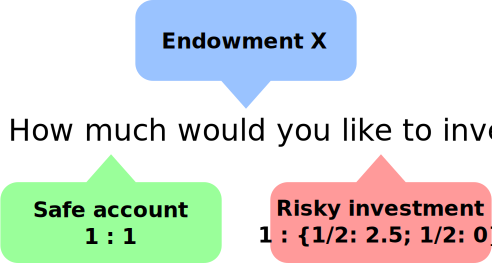
\includegraphics[width=6.25in,height=\textheight]{CGP.png}

\end{frame}

\begin{frame}{Balloon Analog Risk Task (Lejuez et al)}
\protect\hypertarget{balloon-analog-risk-task-lejuez-et-al}{}

\includegraphics[width=3.125in,height=\textheight]{BART.png}

\end{frame}

\begin{frame}{Certainty Equivalent MPL}
\protect\hypertarget{certainty-equivalent-mpl}{}

\includegraphics[width=3.64583in,height=\textheight]{CEPL.png}

\end{frame}

\begin{frame}{CRRA (à la Wakker)}
\protect\hypertarget{crra-uxe0-la-wakker}{}

\(u(x) = x^r\)

\begin{itemize}
\tightlist
\item
  simple
\item
  captures risk aversion
\item
  makes different tasks comparable
\end{itemize}

\end{frame}

\begin{frame}{How big are these differences?}
\protect\hypertarget{how-big-are-these-differences}{}

\includegraphics{Presentation_ESA_files/figure-beamer/unnamed-chunk-1-1.pdf}

\end{frame}

\begin{frame}{Elicited attitudes: summary}
\protect\hypertarget{elicited-attitudes-summary}{}

\begin{itemize}
\item
  \textbf{low} consistency across tasks
\item
  surprisingly, \textbf{low} consistency also \emph{within} tasks
\item
  but \textbf{heterogeneity} by task is large
\item
  only result that holds: most people are \emph{risk averse}
\end{itemize}

\begin{quote}
possible explanation: between-subjects variation.
\end{quote}

\end{frame}

\hypertarget{questionnaires}{%
\section{Questionnaires}\label{questionnaires}}

\begin{frame}{Questionnaires: summary}
\protect\hypertarget{questionnaires-summary}{}

\begin{itemize}
\item
  \textbf{better} consistency across samples
\item
  a tendency to report \emph{`in the middle'}
\item
  we do not really know what those number mean
\end{itemize}

\end{frame}

\hypertarget{convergent-validity-correlations-among-rets}{%
\section{\texorpdfstring{Convergent validity: \textbf{correlations}
among
RETs}{Convergent validity: correlations among RETs}}\label{convergent-validity-correlations-among-rets}}

\begin{frame}{Convergence: more evidence}
\protect\hypertarget{convergence-more-evidence}{}

\begin{figure}
\centering
\includegraphics[width=6.77083in,height=\textheight]{NHB_correlation.png}
\caption{Pedroni et al.~Nature Human Behavior 2017}
\end{figure}

\end{frame}

\begin{frame}{Convergence: summary}
\protect\hypertarget{convergence-summary}{}

\begin{itemize}
\item
  we replicate Slovic 1962 (!!)
\item
  no correlation higher than .35
\item
  when transalitng into r things get \emph{worse}
\end{itemize}

\end{frame}

\hypertarget{predictive-validity-correlation-with-questionnaires}{%
\section{Predictive validity: correlation with
questionnaires}\label{predictive-validity-correlation-with-questionnaires}}

\begin{frame}{Predictive validity: more evidence}
\protect\hypertarget{predictive-validity-more-evidence}{}

\begin{figure}
\centering
\includegraphics[width=7.29167in,height=\textheight]{frey.png}
\caption{Frey et al.~Science Advances 2017}
\end{figure}

\end{frame}

\begin{frame}{Predictive validity: summary}
\protect\hypertarget{predictive-validity-summary}{}

\begin{itemize}
\item
  \textbf{low} correlations with questionnaires
\item
  across questionnaires and tasks
\item
  Beauchamp et al JRU 2016: questionnaires are rather predictive
\end{itemize}

\begin{quote}
\textbf{we have a problem}
\end{quote}

\end{frame}

\hypertarget{why}{%
\section{Why?}\label{why}}

\begin{frame}{Noise}
\protect\hypertarget{noise}{}

\begin{quote}
\emph{noisy} preference + one-shot choices \(\Rightarrow\) noisy data
\end{quote}

\begin{itemize}
\item
  cognitive limits \(\Rightarrow\) limited understanding
\item
  \emph{if} risk preferences fuzzy \(\Rightarrow\) noisy estiamte
\end{itemize}

\begin{quote}
solution: go \textbf{fully structural}
\end{quote}

\begin{itemize}
\tightlist
\item
  Hey and Orme 1994
\item
  Harrison and coauthors (several papers)
\end{itemize}

\begin{quote}
forget quick \& dirty task, embrace complexity
\end{quote}

\begin{quote}
Maximum Likelihood at the \textbf{individual} level
\end{quote}

\end{frame}

\begin{frame}{Risk perception}
\protect\hypertarget{risk-perception}{}

\includegraphics[width=7.29167in,height=\textheight]{risk_def.png}

\end{frame}

\begin{frame}{Risk perception: a mismatch}
\protect\hypertarget{risk-perception-a-mismatch}{}

\begin{itemize}
\item
  economists \emph{assume} subjects share the same risk
  \emph{definition}
\item
  namely:

  \begin{itemize}
  \tightlist
  \item
    risk as a distribution of \textbf{probability} over outcomes
  \item
    \(EV\) as the average across all possible states of the world
  \item
    risk aversion as diminishing marginal utility of money
  \item
    subjects care about \textbf{variance}
  \end{itemize}
\item
  but subjects think of risk as \emph{probability of a loss}
\end{itemize}

\begin{itemize}[<+->]
\tightlist
\item
  \emph{do subjects find our tasks risky?}
\end{itemize}

\begin{itemize}[<+->]
\tightlist
\item
  We \textbf{do not know} because we \textbf{assume} they do
\end{itemize}

\end{frame}

\begin{frame}{Experimenting on risk perception}
\protect\hypertarget{experimenting-on-risk-perception}{}

\begin{itemize}
\tightlist
\item
  Holzmeister et al Working Paper
\item
  gave description of return from an asset to subjects
\item
  \$\sim\$7000 subjects
\item
  including \$\sim\$2500 \textbf{traders}
\item
  asked to rate \textbf{perceived risk of each asset}
\end{itemize}

\end{frame}

\begin{frame}{Holzmeister et al: design}
\protect\hypertarget{holzmeister-et-al-design}{}

\includegraphics[width=6.5625in,height=\textheight]{hm_dist.png}

\end{frame}

\begin{frame}{results - skewness}
\protect\hypertarget{results---skewness}{}

\includegraphics[width=5.20833in,height=\textheight]{skew.png}

\end{frame}

\begin{frame}{results - aggregate risk measures}
\protect\hypertarget{results---aggregate-risk-measures}{}

\includegraphics[width=8.33333in,height=\textheight]{zeisberger.png}

\end{frame}

\hypertarget{roads-ahead}{%
\section{Roads ahead}\label{roads-ahead}}

\begin{frame}{Theory}
\protect\hypertarget{theory}{}

\begin{itemize}
\tightlist
\item
  Spiliopoulos \& Hertwig: \emph{different} \textbf{decision rules} for
  different contexts
\item
  Schneider and Sutter: \textbf{higher moments} matter
\item
  Sunder et al: \emph{curvature of utility} function \textbf{not} a
  valid theory
\item
  \textbf{Ergodicity} economics (peters et al): drop EV, use time-means
\item
  \ldots{}
\end{itemize}

\end{frame}

\begin{frame}{Empirics}
\protect\hypertarget{empirics}{}

\begin{itemize}
\tightlist
\item
  use \textbf{meta-analysis} to find patterns

  \begin{itemize}
  \tightlist
  \item
    do not aggregate \emph{by task} but \textbf{by characteristic}
  \item
    map what correlates and what doesn't
  \end{itemize}
\item
  tackle \textbf{noise} through

  \begin{itemize}
  \tightlist
  \item
    binary chocies among lotteries
  \item
    econometric modeling of noise
  \item
    individual esitmates with MaxLik
  \item
    iterate with Machine Learning to fid best lottery set
  \end{itemize}
\item
  tackle \textbf{perception} rather than assuming it away
\end{itemize}

\end{frame}

\begin{frame}{In a few words\ldots{}}
\protect\hypertarget{in-a-few-words}{}

\begin{itemize}[<+->]
\tightlist
\item
  \emph{``\ldots future research must carefully consider the problem of
  adequately \textbf{defining} and \textbf{assessing} risk taking
  behavior.''}
\end{itemize}

\begin{itemize}[<+->]
\tightlist
\item
  \textbf{exactly as in 1962}
\end{itemize}

\end{frame}

\hypertarget{thanks}{%
\section{Thanks!}\label{thanks}}

\begin{frame}{Contribute to the meta-analysis!}
\protect\hypertarget{contribute-to-the-meta-analysis}{}

\textbf{if}:

\begin{itemize}
\tightlist
\item
  you have \textbf{run a RET}
\item
  you have run \textbf{more} than one
\item
  you have run a RET and a \textbf{questionnaire}
\item
  you have run a RET and another \textbf{risk-related measure}
\end{itemize}

\begin{quote}
send your data --
\href{mailto:paolo.crosetto@inra.fr}{\nolinkurl{paolo.crosetto@inra.fr}}
\end{quote}

\begin{quote}
github: (\url{https://github.com/paolocrosetto/METARET})
\end{quote}

\begin{quote}
shiny app: (\url{https://paolocrosetto.shinyapps.io/METARET/})
\end{quote}

\end{frame}

\end{document}
